\documentclass[12pt,letterpaper]{article}
\usepackage{graphicx,textcomp}
\usepackage{natbib}
\usepackage{setspace}
\usepackage{fullpage}
\usepackage{color}
\usepackage[reqno]{amsmath}
\usepackage{amsthm}
\usepackage{fancyvrb}
\usepackage{amssymb,enumerate}
\usepackage[all]{xy}
\usepackage{endnotes}
\usepackage{lscape}
\newtheorem{com}{Comment}
\usepackage{float}
\usepackage{hyperref}
\newtheorem{lem} {Lemma}
\newtheorem{prop}{Proposition}
\newtheorem{thm}{Theorem}
\newtheorem{defn}{Definition}
\newtheorem{cor}{Corollary}
\newtheorem{obs}{Observation}
\usepackage[compact]{titlesec}
\usepackage{dcolumn}
\usepackage{tikz}
\usetikzlibrary{arrows}
\usepackage{multirow}
\usepackage{xcolor}
\newcolumntype{.}{D{.}{.}{-1}}
\newcolumntype{d}[1]{D{.}{.}{#1}}
\definecolor{light-gray}{gray}{0.65}
\usepackage{url}
\usepackage{listings}
\usepackage{color}
\usepackage{relsize}

\definecolor{codegreen}{rgb}{0,0.6,0}
\definecolor{codegray}{rgb}{0.5,0.5,0.5}
\definecolor{codepurple}{rgb}{0.58,0,0.82}
\definecolor{backcolour}{rgb}{0.95,0.95,0.92}

\lstdefinestyle{mystyle}{
	backgroundcolor=\color{backcolour},   
	commentstyle=\color{codegreen},
	keywordstyle=\color{magenta},
	numberstyle=\tiny\color{codegray},
	stringstyle=\color{codepurple},
	basicstyle=\footnotesize,
	breakatwhitespace=false,         
	breaklines=true,                 
	captionpos=b,                    
	keepspaces=true,                 
	numbers=left,                    
	numbersep=5pt,                  
	showspaces=false,                
	showstringspaces=false,
	showtabs=false,                  
	tabsize=2
}
\lstset{style=mystyle}
\newcommand{\Sref}[1]{Section~\ref{#1}}
\newtheorem{hyp}{Hypothesis}

\title{Problem Set 3}
\date{Due: November 13, 2025}
\author{Rosalie LaCroix}


\begin{document}
	\maketitle
	\section*{Instructions}
	\begin{itemize}
		\item Please show your work! You may lose points by simply writing in the answer. If the problem requires you to execute commands in \texttt{R}, please include the code you used to get your answers. Please also include the \texttt{.R} file that contains your code. If you are not sure if work needs to be shown for a particular problem, please ask.
	\item Your homework should be submitted electronically on GitHub.
	\item This problem set is due before 23:59 on Thursday November 13, 2025. No late assignments will be accepted.

	\end{itemize}

		\vspace{.25cm}
	
\noindent In this problem set, you will run several regressions and create an add variable plot (see the lecture slides) in \texttt{R} using the \texttt{incumbents\_subset.csv} dataset. Include all of your code.

	\vspace{.5cm}
\section*{Question 1}
\vspace{.25cm}
\noindent We are interested in knowing how the difference in campaign spending between incumbent and challenger affects the incumbent's vote share. 
	\begin{enumerate}
		\item Run a regression where the outcome variable is \texttt{voteshare} and the explanatory variable is \texttt{difflog}.
			\lstinputlisting[language=R, firstline=40, lastline=40]{PS03_RL.R}
			\newpage
		\item Make a scatterplot of the two variables and add the regression line. 
			\lstinputlisting[language=R, firstline=45, lastline=49]{PS03_RL.R}
			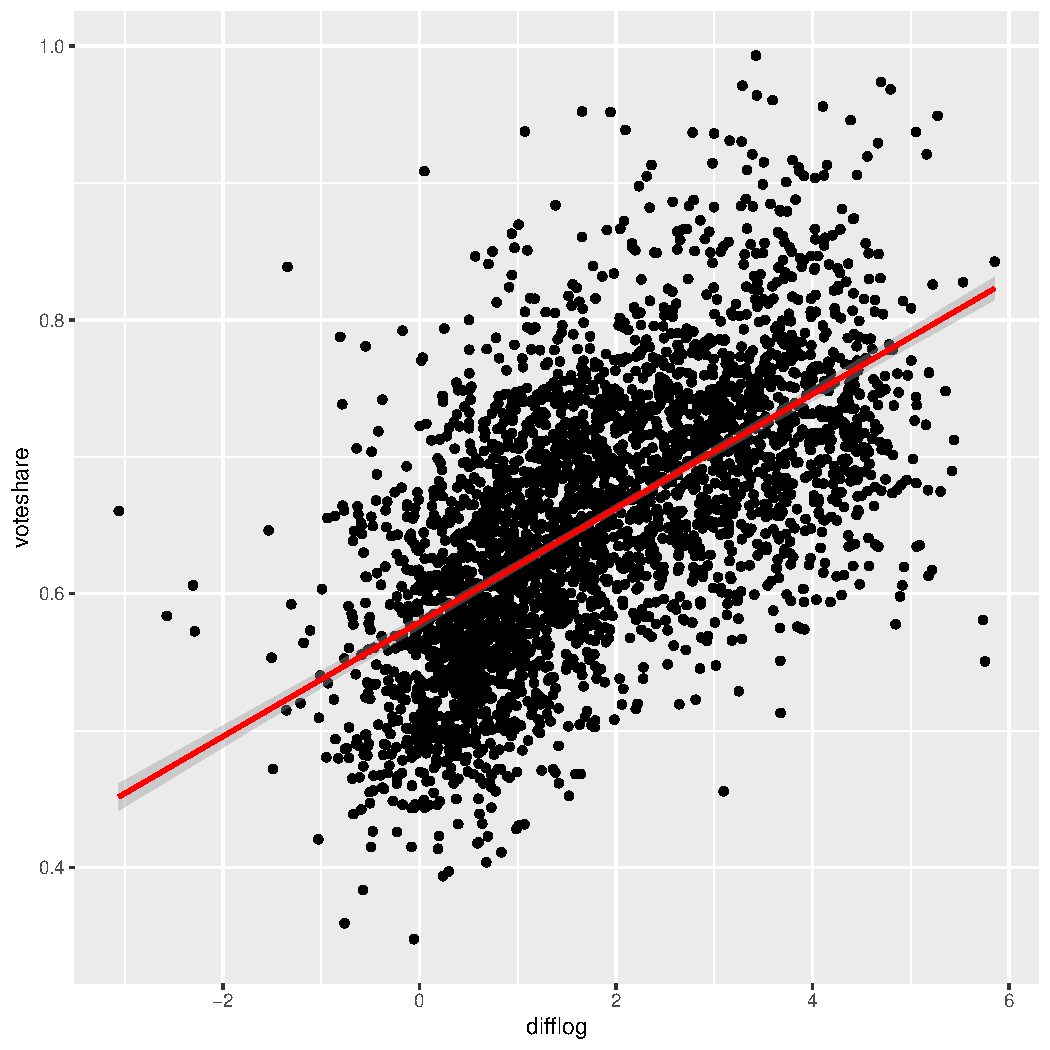
\includegraphics[width=10cm]{scatterplot_1.pdf}
		\item Save the residuals of the model in a separate object.	
		\lstinputlisting[language=R, firstline=53, lastline=53]{PS03_RL.R}
		\item Write the prediction equation.
			\lstinputlisting[language=R, firstline=56, lastline=56]{PS03_RL.R}
			
		\textsmaller[1]{The prediction equation is y = 0.5790 + 0.0417x or voteshare = 0.5790 + 0.0417difflog in the context of this specific data.}
		
	\end{enumerate}
	
\newpage

\section*{Question 2}
\noindent We are interested in knowing how the difference between incumbent and challenger's spending and the vote share of the presidential candidate of the incumbent's party are related.	\vspace{.25cm}
	\begin{enumerate}
		\item Run a regression where the outcome variable is \texttt{presvote} and the explanatory variable is \texttt{difflog}.	
			\lstinputlisting[language=R, firstline=62, lastline=62]{PS03_RL.R}
		\item Make a scatterplot of the two variables and add the regression line. 
			\lstinputlisting[language=R, firstline=67, lastline=71]{PS03_RL.R}
			\includegraphics[width=10cm]{scatterplot_2.pdf}
		\item Save the residuals of the model in a separate object.	
			\lstinputlisting[language=R, firstline=75, lastline=75]{PS03_RL.R}
		
		\newpage
		\item Write the prediction equation.
			\lstinputlisting[language=R, firstline=78, lastline=78]{PS03_RL.R}
			
		\textsmaller[1]{The prediction equation is y = 0.5076 + 0.0238x or presvote = 0.5076 + 0.0238difflog in the context of this specific data.}
		
	\end{enumerate}
	
	\newpage	
\section*{Question 3}

\noindent We are interested in knowing how the vote share of the presidential candidate of the incumbent's party is associated with the incumbent's electoral success.
	\vspace{.25cm}
	\begin{enumerate}
		\item Run a regression where the outcome variable is \texttt{voteshare} and the explanatory variable is \texttt{presvote}.
			\lstinputlisting[language=R, firstline=84, lastline=84]{PS03_RL.R}
		\item Make a scatterplot of the two variables and add the regression line. 
			\lstinputlisting[language=R, firstline=89, lastline=93]{PS03_RL.R}
			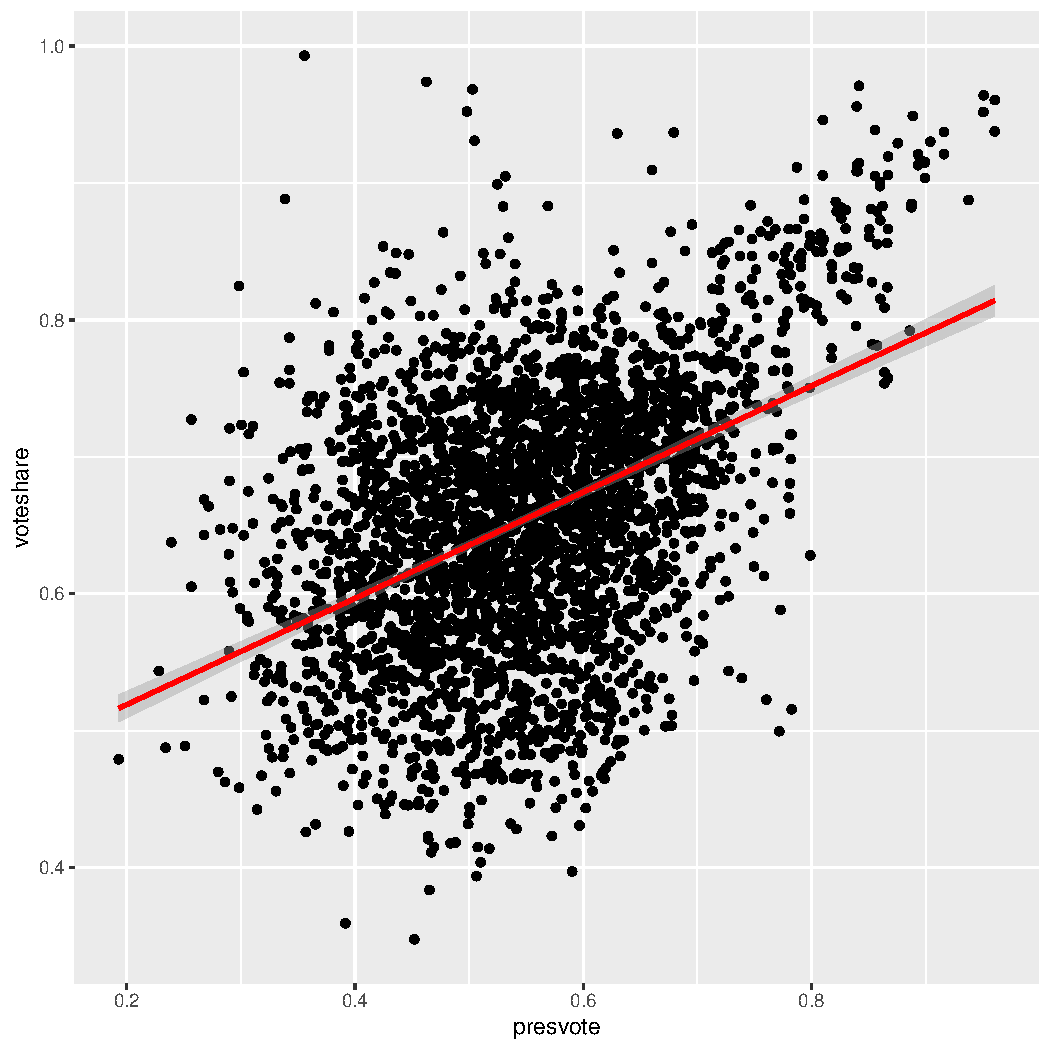
\includegraphics[width=10cm]{scatterplot_3.pdf}
		
		\newpage
		\item Write the prediction equation.
			\lstinputlisting[language=R, firstline=97, lastline=97]{PS03_RL.R}
			
		\textsmaller[1]{The prediction equation is y = 0.4413 + 0.3880x or voteshare = 0.4413 + 0.3880presvote in the context of this specific data.}
		
	\end{enumerate}
	

\newpage	
\section*{Question 4}
\noindent The residuals from part (a) tell us how much of the variation in \texttt{voteshare} is $not$ explained by the difference in spending between incumbent and challenger. The residuals in part (b) tell us how much of the variation in \texttt{presvote} is $not$ explained by the difference in spending between incumbent and challenger in the district.
	\begin{enumerate}
		\item Run a regression where the outcome variable is the residuals from Question 1 and the explanatory variable is the residuals from Question 2.
			\lstinputlisting[language=R, firstline=103, lastline=103]{PS03_RL.R}
		\item Make a scatterplot of the two residuals and add the regression line. 
			\lstinputlisting[language=R, firstline=107, lastline=113]{PS03_RL.R}
			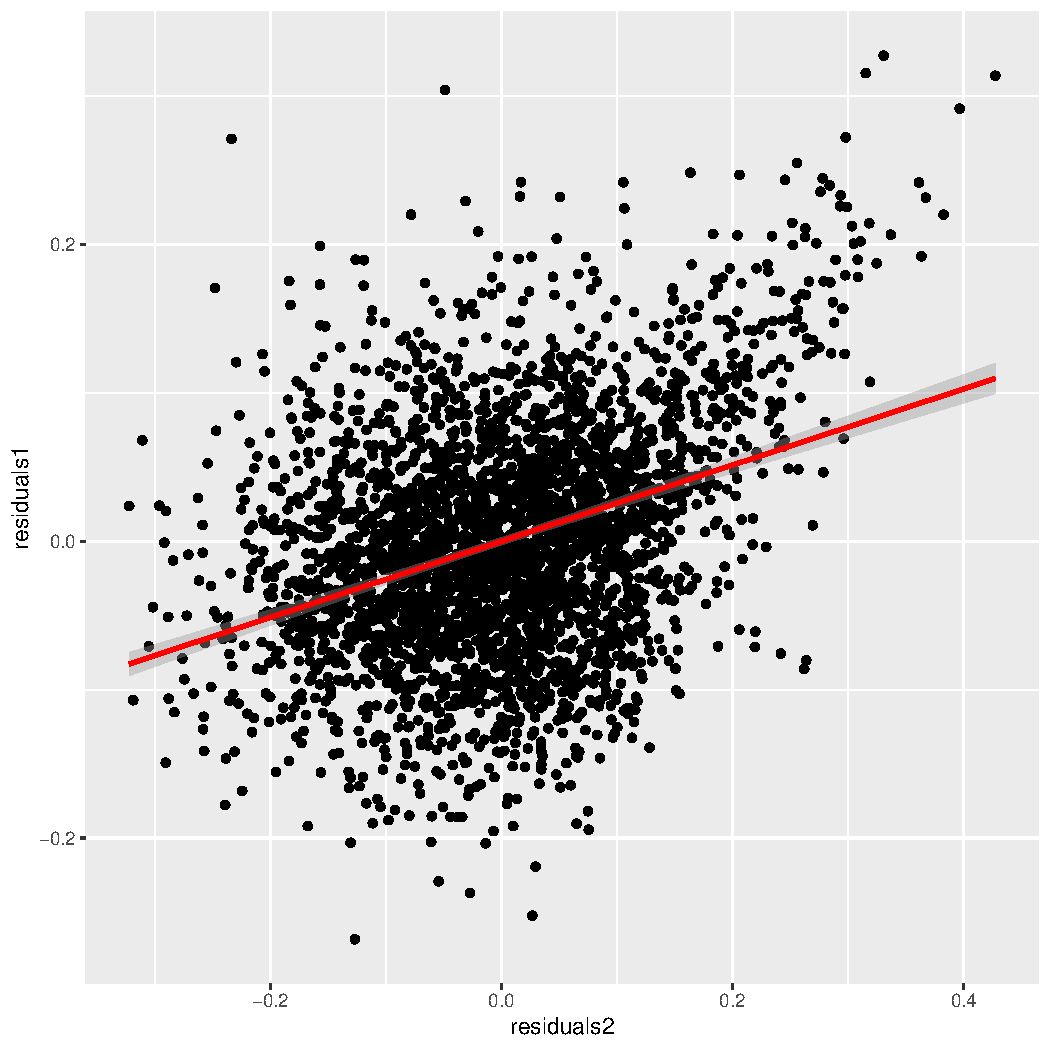
\includegraphics[width=10cm]{scatterplot_4.pdf}
		\item Write the prediction equation.
		
		\textsmaller[1]{The prediction equation is y = -1.942e-18 + 0.2569x or residuals1 = -1.942e-18 + 0.2569residuals2 in the context of this specific data.}
	\end{enumerate}
	
	\newpage	

\section*{Question 5}
\noindent What if the incumbent's vote share is affected by both the president's popularity and the difference in spending between incumbent and challenger? 
	\begin{enumerate}
		\item Run a regression where the outcome variable is the incumbent's \texttt{voteshare} and the explanatory variables are \texttt{difflog} and \texttt{presvote}.
			\lstinputlisting[language=R, firstline= 123, lastline= 123]{PS03_RL.R}
		\item Write the prediction equation.
			\lstinputlisting[language=R, firstline=127, lastline=127]{PS03_RL.R}
			\textsmaller[1]{The prediction equation is y = 0.4486 + 0.0355$x_{1}$ + 0.2569$x_{2}$ or voteshare = 0.4486 + 0.0355difflog + 0.2569presvote in the context of this specific regression.}
		\item What is it in this output that is identical to the output in Question 4? Why do you think this is the case?
			
			\textsmaller[1]{In this output and in the output in Question 4, the slope for presvote impact on voteshare is identical to the slope for residuals2 impact on residuals1, which are both 0.2569. These two values are the same as they represent the same thing. Residuals2 represents the variation in incumbent's vote share (electoral success) that is not explained by the difference in spending between incumbent and challenger, which is subsequently the variation in incumbent's vote share that is explained by the vote share of the presidential candidate of the incumbent's party, which is represented by presvote in the final equation. This can be concluded, as the outcome variable in the final equation is incumbent vote share and the two explanatory variables are difference in spending between incumbent and challenger and vote share of the presidential candidate of the incumbent's party. The impact of vote share of the presidential candidate of the incumbent's party is therefore equal to the variation in vote share that is not attributed to the other explanatory variable of difference in spending between incumbent and challenger.}
			
			Voteshare = incumbent's vote share (electoral success)
			difflog = difference in campaign spending between incumbent and challenger
			presvote = vote share of the presidential candidate of the incumbent's party
			Residuals1 = variation in incumbent's vote share not explained by the difference in spending between incumbent and challenger
			residuals2 = variation in the vote share of the presidential candidate of the incumbent's party not explained by the difference in spending between incumbent and challenger in the district
			For a one unit increase in the variation in presvote not explained by the difference in spending between incumbent and challenger, variation in voteshare that is not explained by the difference in spending between incumbent and challenger increases by 0.2569. 
			
			Residuals2 = variation in presvote not explained by the variation in diff log
			For every one unit increase in variation in presvote not explained by diff log, variation in voteshare not explained by diff log increases by 0.2569
			
			When the vote share of the presidential candidate of the incumbent's party increases by 1, the incumbent's vote share increases by 0.2569, which is the variation in the incumbent's vote share that is explained by the presvote variable and therefore can not be attributed to changes in the difflog variable. Similarly in regards to the residuals, when the variation in vote share of the presidential candidate that cannot be attributed to the difference in spending between incumbent and challenger increases by 1 (just the variation in presidental candidate of the incumbent's party vote share), the variation in the incumbent's vote share the cannot be attributed to the difference in spending increases by 0.2569. 
			
	\end{enumerate}




\end{document}
